\documentclass[9pt,t,xcolor=table]{beamer}
\usetheme{kuleuven2}
\usepackage[english]{babel}
\usepackage{amsfonts}
\usepackage{amssymb}
\useinnertheme{circles}
\usefonttheme[onlymath]{serif}	
\usepackage{mathtools}
\usepackage{amsmath}
\setbeamertemplate{footline}[body]
\usepackage{physics}
\usepackage{chemfig}
\usepackage{graphicx}
\usepackage{mdframed}
\usepackage{cancel}
\usepackage{textcomp}
\usepackage{xcolor}
\usepackage[english]{babel}
\usepackage{soul}
\usepackage{setspace}
\usepackage{fancyvrb}
\usepackage[export]{adjustbox}
\usepackage{mathtools,booktabs,amsmath,upgreek,amsfonts,amssymb,multirow,tikz}
\usepackage[utf8]{inputenc}
\usepackage{csquotes}
\usepackage[absolute, overlay]{textpos}
\usepackage[T1]{fontenc}
\usepackage{pgfplots}
\pgfplotsset{compat=1.18}
\def\Put(#1,#2)#3{\leavevmode\makebox(0,0){\put(#1,#2){#3}}}

\title{Exploring biologically relevant non-valence anions with the CC2 method}
\subtitle{TCCM}
%\author{Mauro Gascón Navas}
\author{Mauro Gascón Navas \\ Promotor: Prof. Thomas Jagau \\ Supervisor: Robin Moorby}
%\institute{Prof. Thomas Jagau}
\date{February 24, 2025}
\renewcommand\fbox{\fcolorbox{blue}{white}}

\begin{document}

% title frame
\begin{frame}[plain,noframenumbering]
	\titlepage
	\Put(150,-535){\includegraphics[width=0.6\textwidth]{Figs/uQ.png}}
\end{frame}

\begin{frame}{\huge Outline}\large
	\vspace{5pt}
	\centering
	\begin{itemize}
		\item \textbf{Background}
		\item Non-Valence anions
		\item Equation-of-Motion CC
		\item Ubiquinone
		\item \textbf{Results}
		\item Dipole Surface
		\item A Simple Cluster Model
		\item \textbf{Future steps} 
	\end{itemize}
\end{frame}

\begin{frame}{\huge Non-Valence anions}\large
	In non-valence anions (NVAs) the excess electron resides in a diffuse orbital stabilized by long-range interactions
	\vspace{5pt}
	\begin{itemize} 
		\item Relevant for electron scattering and transfer processes and can act as a doorway for a valence state
		\item Require huge basis sets and accurate correlation treatment
	\end{itemize}
	\vspace{5pt}
	\begin{columns}
		\begin{column}{0.27\textwidth}
			\centering
			\includegraphics[width=\textwidth]{Figs/vbaDNA.png}
			G valence anion
		\end{column}
		\begin{column}{0.3\textwidth}
			\centering
			\includegraphics[width=\textwidth]{Figs/dbaDNA.png}
			G dipole anion
		\end{column}
		\begin{column}{0.27\textwidth}
			\centering
			\includegraphics[width=\textwidth]{Figs/hf3.png}
			(HF)\textsubscript{3} solvated electron
		\end{column}	
	\end{columns}
	\vspace{5pt}
	\tiny Dutta, A. Int. J. of Quant. Chem., 2015\\
	Gutowski, M., Phy. Rev. Let., 2002
\end{frame}

\begin{frame}{\huge EOM-EA}\large
	Equation-of-motion electron-attachment coupled-cluster (EOM-EA-CC) methods are particularly well suited to study NVAs
	\vspace{5pt}
	\begin{itemize}
		\item The description is based on the wavefunction of the parent neutral molecule
		\item The computational cost and memory requirements limit the EOM-EA-CCSD applications to small molecules
	\end{itemize}
	\begin{columns}
		\begin{column}{0.4\textwidth}
			\vspace{5pt}
			\includegraphics[width=\textwidth]{Figs/EAdiag.pdf}
		\end{column}

		\begin{column}{0.60\textwidth}
			\vspace{25pt} \centering
			\[ \hat{R}_{\mathrm{EA}} = \sum_{a} r^a a_a^\dagger + \frac{1}{2} \sum_{ab} \sum_{i} r_{i}^{ab} a_a^\dagger a_i a_b^\dagger + \dots \]
		\end{column}	
	\end{columns}
\end{frame}

\begin{frame}{\huge CC2}\large
	Second-order approximate coupled-cluster singles and doubles (CC2) method is obtained from a perturbative analysis of the CCSD model
	\vspace{5pt}
	\begin{itemize}
		\item Lowers computational scaling from CCSD 
		\item Allows treatment of “big” molecules: $>$ 25 heavy atoms
	\end{itemize}
	\centering
	\vspace{30pt}
	\begin{table}
		\centering
		\begin{tabular}{lcc}\toprule
		\textbf{Method} & \textbf{Scaling} & \textbf{Memory}\\\midrule
		CCSD & $O(N^6)$ & $O(N^{4})^*$\\
		CC2 & $O(N^5)$ & $O(N^{4})^*$\\\bottomrule
		\multicolumn{3}{l}{\small $^*\,O(N^3)$ with RI approximation.}
		\end{tabular}
	\end{table}
\end{frame}

\begin{frame}{\huge Biological Quinones: Ubiquinone (CoQ)}\large
	Quinones are essential electron carriers in biological mechanisms
	\vspace{5pt}
	\begin{itemize}
	%	\item Ubiquinone (coenzyme Q or CoQ) is a component of electron transport chains in bacterial photosynthesis and aerobic respiration.
	\item CoQ: component of electron transport chains in bacterial photosynthesis and aerobic respiration	
	\item It is capable of both a valence and dipole bound anion states
	\end{itemize}
	\Put(140,-285){\includegraphics[width=0.55\textwidth]{Figs/uQ_6i0d.png}}	
	\Put(235,-110){\includegraphics[width=0.25\textwidth]{Figs/Ubiquinone–ubiquinol_conversion.svg.png}}	
	\Put(0,-265){\includegraphics[width=0.45\textwidth]{Figs/Mitochondrial_electron_transport_chain—Etc4.svg.png}}
	\Put(80,-225){\fontsize{4.5}{4}\selectfont\color{darkgray}\text{Ref: Wikimedia Commons}}
	\Put(238,-285){\fontsize{4.5}{4}\selectfont\color{darkgray}\text{PDB: 6i0d}}

\end{frame}

\begin{frame}{\huge Quinone models}\large
	\begin{itemize}
		\item Quinone head involved in the electron transfer
		\item Isoprenoid tail responsible for the solubility in the membrane
		\item Methoxy chains determine the dipole moment
	\end{itemize}
	\Put(-30,-265){\includegraphics[width=0.55\textwidth]{Figs/uQ_6i0d.png}}
	\Put(85,-285){\includegraphics[width=0.57\textwidth]{Figs/Q1.png}}
	\Put(200,-238){\includegraphics[width=0.465\textwidth]{Figs/Q0189.png}}

	\Put(20,-265){\fontsize{8}{4}\selectfont\text{Q10, Cluster Model}}
	\Put(165,-265){\fontsize{8}{4}\selectfont\color{darkgray}\text{Q1}}
	\Put(270,-265){\fontsize{8}{4}\selectfont\color{darkgray}\text{Q0}}
\end{frame}

\begin{frame}{\Huge Objectives}\large
	\begin{itemize}
		\item Characterize dipole bound state for different CoQ models and conformations
		\item Explore effect of enviroment
		\item Possible involvement in charge transfer reactions
	\end{itemize}	
	\vspace{10pt}
	\Huge\textcolor{kul-blue}{\textbf{Computational methods}}
	\large
	\vspace{5pt}
	\begin{itemize}
		\item Optimizations performed at TPSS+D3BJ/ma-def2-TZVP
		EA calculated at the RI-EOM-EA-CC2 using the neutral ground state as CC reference state
		\item aug-cc-pVTZ or DVZ basis further augmented by 3 s-shells on Hydrogen atoms and 6 s- and 3 p-shells on all non-hydrogen atoms
	\end{itemize}
	\vspace{5pt}
	\centering
	\includegraphics[width=0.3\textwidth]{Figs/QCLogo.png}
\end{frame}

\begin{frame}{\huge Q0 Dipole PES}\large
	Simmilarly to a Potential Energy Surface (PES), we can construct a Dipole Moment Surface (DMS) for the Q0 model.
	\vspace{5pt}
	\begin{itemize}
		\item $\Psi$ and $\Phi$ are the methoxy dihedrals.
	\end{itemize}
	\vspace{5pt}
	\includegraphics[width=1\textwidth]{Figs/PES.png}
	\Put(229,337){\includegraphics[width=0.45\textwidth]{Figs/dihedrals.png}}
\end{frame}

\begin{frame}{\huge Q0 Dipole PES}\large
	Dipole strength is not the whole picture
	\begin{columns}
		\begin{column}{0.5\textwidth}
			\centering
			\includegraphics[width=0.7\textwidth]{Figs/Q0_181.png} \\
			{\textmu} 2.4 D EA\textsubscript{dba} +12.3 meV \\
			
			\includegraphics[width=0.7\textwidth]{Figs/Q0_90.png} \\
			{\textmu} 3.2 D EA\textsubscript{dba} +4.7 meV
		\end{column}
		\begin{column}{0.5\textwidth}
			\centering
			\includegraphics[width=0.7\textwidth]{Figs/Q0_6.png} \\
			{\textmu} 2.8 D EA\textsubscript{dba} +3.6 meV \\
			
			\includegraphics[width=0.7\textwidth]{Figs/Q0_360.png} \\
			{\textmu} 0.5 D EA\textsubscript{dba} -7.9 meV
		\end{column}
	\end{columns}
\end{frame}

\begin{frame}{\huge A simple cluster model}\large
	Encase Q0 in a Helium icosahedron.
	\vspace{5pt}
	\begin{itemize}
		\item Valence state gets stabilized by the "solvent"
		\item Dipole state gets destabilized
	\end{itemize}
	%\vspace{5pt}
	\Put(60,-220){\includegraphics[width=0.25\textwidth]{Figs/He6.png}}
	\Put(200,-190){\includegraphics[width=0.465\textwidth]{Figs/He20.png}}
	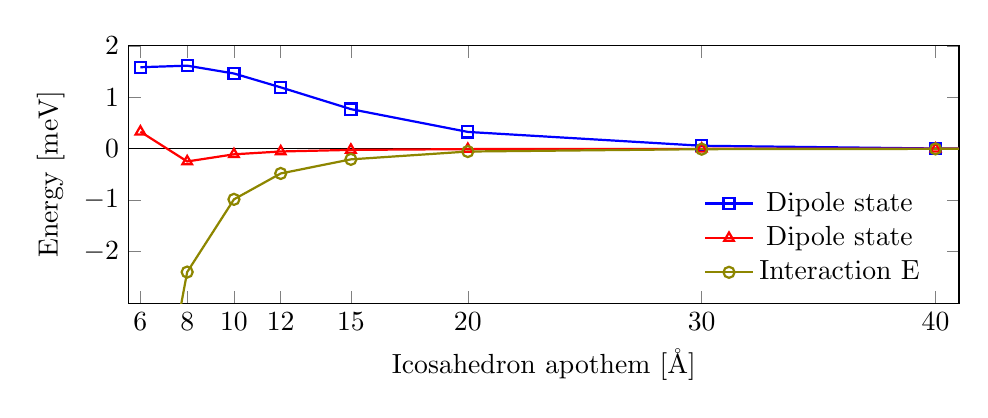
\begin{tikzpicture}
    \begin{axis}[
        width=1\textwidth,
        height=0.4\textwidth,
        ylabel={Energy [meV]},
        xlabel={Icosahedron apothem [\r{A}]},
        xmin=5.5, xmax=41,
        ymin=-3, ymax=2,
        xtick={6,8,10,12,15,20,30,40},
        ytick={0,-1, 1,-2,2},
        legend pos=south east,
        legend style={draw=none,fill=none}
    ]
    \draw ({rel axis cs:0,0}|-{axis cs:0,0}) -- ({rel axis cs:1,0}|-{axis cs:0,0});
    \draw ({rel axis cs:0,0}-|{axis cs:0,0}) -- ({rel axis cs:0,1}-|{axis cs:0,0});

    \addplot[
    color=blue,
    mark=square,
    line width=0.8pt
    ]
    coordinates {
        (6,1.584) (8,1.614) (10,1.462) (12,1.193) 
        (15,0.770) (20,0.327) (30,0.058) (40,0.005) (50,0.000)
    };
    \addlegendentry{Dipole state}

    \addplot[
        color=red,
        mark=triangle,
        line width=0.8pt
    ]
    coordinates {
        (6,0.331) (8,-0.247) (10,-0.108) (12,-0.053) 
        (15,-0.022) (20,-0.007) (30,-0.002) (40,-0.001) (50,0.000)
    };
    \addlegendentry{Dipole state}

    \addplot[
        color=olive,
        mark=o,
        line width=0.8pt
    ]
    coordinates {
        (6,-7.255) (8,-2.396) (10,-0.983) (12,-0.480) 
        (15,-0.206) (20,-0.054) (30,-0.008) (40,-0.002) (50,0.000)
    };
    \addlegendentry{Interaction E}
    \end{axis}
    \end{tikzpicture}
\end{frame}

\begin{frame}{\huge Future steps}\large
	\begin{itemize}
		\item More realistic cluster model: polar residues might help “solvate” the electron
		\item Effect of isoprenoid tail
		\item Study other species: plastoquinone, vitamin K		
	\end{itemize}
	\centering
	\vspace{40pt}
	\Huge \textcolor{kul-blue}{\textbf{Thanks for your attention!}}
\end{frame}

\begin{frame}{\huge Basis set convergence}\large
	Basis size and \# of extra diffuse functions effect on dipole bound states\\
	\begin{table}[h!]
		\centering
		\footnotesize
		\begin{tabular}{lccccc}
		 & \multicolumn{3}{c}{RI-CC2} & \multicolumn{2}{c}{RI-CCSD} \\
		\cmidrule(lr){2-4} \cmidrule(lr){5-6}
		 & pVDZ+6s3p & pVTZ+6s3p & pQDZ+6s3p & pVDZ+6s3p & pVTZ+6s3p \\
		\midrule
		acetaldehide & 4.6 & 3.2 & 3.2 & 4.6 & 3.1 \\
		acetone & 0.3 & -1.3 & -0.9 & 0.5 & -0.9 \\
		acetonitrile & -18.2 & -19.9 & -20.3 & -17.1 & -18.4 \\
		benzaldehide & 7.4 & 8.9 & 9.1 & 3.4 & 4.6 \\
		dimethylformamide & 13.2 & 14.1 & 14.4 & 13.3 & 13.7 \\
		dmso & 14.8 & 15.4 & 15.5 & 14.7 & 14.9 \\
		formamide & -16.1 & -16.2 & -17.0 & -15.1 & -15.9 \\
		methylisocyanide & -9.5 & -10.0 & -10.1 & -8.8 & -9.0 \\
		nitrobenzene & -32.5 & -34.8 & - & -28.0 & -25.9 \\
		nitromethane & -13.0 & -14.2 & -14.7 & -12.9 & -13.7 \\
		nitrosobenzene & -9.9 & -11.4 & - & -5.1 & -6.0 \\
		phenylisocyanide & -15.2 & -16.3 & -16.7 & -9.0 & -9.2 \\
		pyridazine & -26.0 & -26.3 & -26.7 & -18.6 & -19.1 \\
		vinylene carbonate& -26.4 & -27.2 & -27.7 & -25.1 & -25.5 \\
		\midrule
		\textbf{MAE} & \textbf{2.3} & \textbf{2.8} & \textbf{2.4} & \textbf{0.8} & \textbf{-} \\
		\bottomrule
		\end{tabular}
	\end{table}
\end{frame}

\begin{frame}{\huge Q0 Dipole PES}\large
	\centering
	\includegraphics[width=0.7\textwidth]{Figs/PES_XYZ.png}
	\Put(-310,340){\includegraphics[width=0.3\textwidth]{Figs/Q0189.png}}
	\Put(-265,280){\includegraphics[width=0.05\textwidth]{Figs/xyzAXIS.pdf}}
\end{frame}

\begin{frame}{\huge Computational methods}\large
	\vspace{5pt}
	\begin{itemize}
		\item Optimizations performed at TPSS+D3BJ/ma-def2-TZVP
		EA calculated at the RI-EOM-EA-CC2 using the neutral ground state as CC reference state
		\item aug-cc-pVTZ basis further augmented by 3 s-shells on Hydrogen atoms and 6 s- and 3 p-shells on all non-hydrogen atoms
	\end{itemize}
	\vspace{35pt}
	\centering
	\includegraphics[width=0.5\textwidth]{Figs/QCLogo.png}
\end{frame}

\end{document}
